%% ============================================================================
%% SSP IEEE Conference Paper
%% Title: Context-Switch and Scheduling Performance Analysis on Multicore
%%        Processors Under Varied Workload Conditions: A Scaling and
%%        Microarchitecture Study
%% Format: IEEE conference (two-column)
%% Compile: pdflatex → bibtex → pdflatex × 2
%% ============================================================================
\documentclass[conference]{IEEEtran}

%% ── Packages ─────────────────────────────────────────────────────────────────
\usepackage[T1]{fontenc}
\usepackage[utf8]{inputenc}
\usepackage{microtype}
\usepackage{cite}
\usepackage{amsmath,amssymb}
\usepackage{graphicx}
\usepackage{booktabs}
\usepackage{array}
\usepackage{url}
\usepackage{xcolor}
\usepackage{balance}      % balance the last two columns
\usepackage{hyperref}
\hypersetup{colorlinks=true,linkcolor=blue,citecolor=blue,urlcolor=blue}

%% ── Metadata ─────────────────────────────────────────────────────────────────
\title{Context-Switch and Scheduling Performance Analysis on Multicore Processors
       Under Varied Workload Conditions: A Scaling and Microarchitecture Study}

\author{
  \IEEEauthorblockN{Shikhar Mutta}
  \IEEEauthorblockA{
    Department of Computer Science and Engineering\\
    Indian Institute of Technology\\
    \textit{shikhar@example.edu}}
}

\begin{document}
\maketitle

%% ═══════════════════════════════════════════════════════════════════════════
%% ABSTRACT
%% ═══════════════════════════════════════════════════════════════════════════
\begin{abstract}
Context switching is a fundamental operating-system primitive whose latency
directly governs the responsiveness of concurrent applications on modern
multicore processors.  Despite decades of research, the interaction between
scheduling overhead, workload contention, and hardware microarchitecture
remains poorly quantified outside controlled laboratory settings.
This paper presents a systematic empirical study of context-switch latency
on an Intel Core i5-1035G1 (Ice Lake, 4 cores/8 threads) using the
\textit{lmbench} \texttt{lat\_ctx} microbenchmark.
We vary three independent dimensions simultaneously: (i)~the number of
active CPU cores (1, 2, 4), (ii)~the number of concurrently switching
processes (2–64), and (iii)~the type and intensity of background system
load (CPU-bound, I/O-bound, memory-bound, and mixed at 25–100\,\%).
Our results show that memory-bound interference inflates context-switch
latency by up to 3.1$\times$ over the idle baseline, while restricting
scheduling to a single core incurs a further 1.45$\times$ overhead.
We attribute these effects to LLC eviction pressure, TLB shootdowns, and
scheduler run-queue contention, providing a clear microarchitecture-level
explanation corroborated by published cache-hierarchy specifications.
\end{abstract}

\begin{IEEEkeywords}
context switching, scheduling latency, multicore, lmbench, workload
characterization, performance analysis, microarchitecture
\end{IEEEkeywords}

%% ═══════════════════════════════════════════════════════════════════════════
%% 1. INTRODUCTION
%% ═══════════════════════════════════════════════════════════════════════════
\section{Introduction}

Modern operating systems achieve concurrent execution by rapidly multiplexing
a finite set of processor cores among many runnable threads.  Each such
\emph{context switch} requires saving and restoring register files, updating
the program counter and stack pointer, and --- critically --- invalidating or
warming up micro-architectural state such as branch-predictor histories,
Translation Lookaside Buffer (TLB) entries, and cache lines.  While the
\emph{direct} cost of a switch is on the order of a few microseconds for the
kernel bookkeeping alone, the \emph{indirect} cost of re-warming caches can
dominate by an order of magnitude, especially when processes hold large working
sets~\cite{li2007quantifying}.

On multicore processors the problem is compounded: the Completely Fair
Scheduler (CFS) must balance load across cores, risking process migration that
carries an additional cache-migration penalty~\cite{lozi2016linux}.  Shared
last-level caches (LLC) and memory buses mean that a CPU-intensive or
memory-intensive co-runner can evict the paused process's cache lines,
inflating the next dispatch's warm-up time even without an explicit
migration~\cite{blagodurov2011numa}.

\textbf{Contributions.}  This work makes the following contributions:
\begin{itemize}
  \item A cross-platform benchmark harness (\textsc{SSP-Bench}) that drives
        \texttt{lmbench lat\_ctx} under programmable background workloads with
        fine-grained intensity control, with a portable Python fallback for
        Windows environments.
  \item A three-dimensional scaling study: core count $\times$ process count
        $\times$ workload intensity, yielding 5-dimensional result surfaces.
  \item A microarchitecture-level explanation of observed trends grounded in
        the Ice Lake cache hierarchy specifications.
\end{itemize}

\textbf{Paper organisation.}
Section~\ref{sec:related} surveys related work.
Section~\ref{sec:background} introduces lmbench and context-switch mechanics.
Section~\ref{sec:methodology} describes the experimental methodology.
Section~\ref{sec:results} presents and interprets results.
Section~\ref{sec:conclusion} concludes.

%% ═══════════════════════════════════════════════════════════════════════════
%% 2. BACKGROUND
%% ═══════════════════════════════════════════════════════════════════════════
\section{Background}
\label{sec:background}

\subsection{Context Switching and Scheduling}
When the OS preempts a running thread, it (1) saves the architectural state
(GPRs, FPRs, SSE/AVX registers, control registers) into the kernel's
\texttt{task\_struct}; (2) selects a new runnable thread via the scheduler
policy; (3) restores that thread's state; and (4) performs an \texttt{iret}
to resume user-mode execution.  The ``direct'' cost is dominated by steps~1
and~3, while the ``indirect'' cost stems from TLB flushes on address-space
switches and cold-start misses in the L1/L2 caches.

CFS, the default Linux scheduler since kernel 2.6.23, computes a
\emph{virtual runtime} (\texttt{vruntime}) for each task, always selecting the
task with the smallest vruntime from a red-black tree.  Its scheduling
granularity (\texttt{sched\_latency\_ns}, default~6\,ms) defines how often a
preemption is forced.

\subsection{The lmbench Microbenchmark Suite}
\texttt{lmbench}~\cite{mcvoy1996lmbench} is an open-source POSIX microbenchmark
suite designed to measure the fundamental cost of OS primitives.
\texttt{lat\_ctx} measures context-switch latency by creating $N$ processes
connected in a token ring via pipes.  A token is passed around the ring; the
time for $K$ full laps divided by $N \cdot K$ yields the per-switch
latency in microseconds.  A ``-s \textit{size}'' flag pre-faults
$\mathit{size}$\,KB of memory in each process to model different working-set
sizes, directly simulating cache pressure.

%% ═══════════════════════════════════════════════════════════════════════════
%% 3. RELATED WORK
%% ═══════════════════════════════════════════════════════════════════════════
\section{Related Work}
\label{sec:related}

\textbf{lmbench (McVoy \& Staelin, 1996).}
The seminal paper introducing lmbench~\cite{mcvoy1996lmbench} established the
token-ring methodology for context-switch measurement and reported latencies
of 15--120\,$\mu$s on 1990s hardware, providing a baseline for comparing
subsequent processor generations.

\textbf{Quantifying Context-Switch Overhead (Li et al., 2007).}
Li \textit{et al.}~\cite{li2007quantifying} decomposed switching cost into
direct (kernel bookkeeping: 1.2--1.5\,$\mu$s) and indirect (cache warm-up:
up to 50\,$\mu$s for large working sets) components, highlighting that LLC
capacity is the principal determinant of the indirect cost.

\textbf{The Linux Scheduler: A Decade of Wasted Cores (Lozi et al., 2016).}
Lozi \textit{et al.}~\cite{lozi2016linux} demonstrated that subtle bugs in
the CFS load-balancer resulted in idle cores while runnable threads were
queued for busy cores.  Their work underscores the importance of empirically
validating scheduler behaviour rather than relying solely on code analysis.

\textbf{NUMA-Aware Contention Management (Blagodurov et al., 2011).}
Blagodurov \textit{et al.}~\cite{blagodurov2011numa} showed that shared-LLC
contention between co-located workloads can reduce IPC by up to 70\%, and
proposed contention-aware placement policies.  Their findings directly motivate
our workload-interference experiments.

\textbf{System-Level Performance Metrics (Eyerman \& Eeckhout, 2008).}
Eyerman and Eeckhout~\cite{eyerman2008system} introduced weighted speedup and
harmonic mean IPC as metrics for evaluating multiprogrammed workload
performance, providing the theoretical grounding for our intensity-vs-latency
analysis framework.

%% ═══════════════════════════════════════════════════════════════════════════
%% 4. METHODOLOGY
%% ═══════════════════════════════════════════════════════════════════════════
\section{Methodology}
\label{sec:methodology}

\subsection{System Under Test}
Experiments ran on a laptop equipped with an Intel Core i5-1035G1 processor
(Ice Lake, 10\,nm, 4 cores / 8 threads, base 1.0\,GHz, boost 3.6\,GHz).
The CPU features 48\,KB L1d / 32\,KB L1i per core, 512\,KB private L2 per
core, and a 6\,MB shared L3 (LLC).  The system runs Ubuntu 22.04 with Linux
kernel 6.5.  Table~\ref{tab:sysconfig} summarises the configuration.

\begin{table}[h]
\centering
\caption{System Configuration}
\label{tab:sysconfig}
\begin{tabular}{ll}
\toprule
\textbf{Parameter} & \textbf{Value} \\
\midrule
CPU                & Intel Core i5-1035G1 @ 1.0/3.6\,GHz \\
Microarchitecture  & Ice Lake (10\,nm) \\
Cores / Threads    & 4 / 8 \\
L1d / L1i (per core)& 48\,KB / 32\,KB \\
L2 (per core)      & 512\,KB \\
L3 (shared)        & 6\,MB \\
DRAM               & 24\,GB DDR4-3200 \\
OS / Kernel        & Ubuntu 22.04 / Linux 6.5 \\
lmbench version    & 3.0-a9 \\
\bottomrule
\end{tabular}
\end{table}

\subsection{Benchmark Harness}
We developed \textsc{SSP-Bench}, a Python orchestration framework that
(a) pins the benchmark process to the first $C$ logical CPUs using
\texttt{taskset}, (b) launches $W$ background load-generator workers
(Python subprocesses), and (c) invokes \texttt{lat\_ctx -s $D$ $N$} with
$D$\,KB context size and $N$ processes.  Each configuration is repeated three
times; the maximum sample is discarded as an outlier, and the remaining two
are averaged.  Source code is available in the project repository.

\subsection{Independent Variables}
\begin{itemize}
  \item \textbf{Active cores} $C \in \{1, 2, 4\}$: enforced via
        CPU-affinity mask (\texttt{taskset}).
  \item \textbf{Process count} $N \in \{2,4,8,16,32,64\}$: fed directly
        to \texttt{lat\_ctx}.
  \item \textbf{Context data size} $D \in \{0,16,64\}$\,KB: models
        increasing working-set sizes relative to L1/L2 capacity.
  \item \textbf{Workload type}: idle baseline; CPU-bound (arithmetic loop);
        I/O-bound (repeated 128\,KB file write/read/fsync); memory-bound (strided
        512\,MB array traversal); mixed (CPU + memory).
  \item \textbf{Workload intensity} $I \in \{25,50,75,100\}$\,\%: duty-cycle
        fraction for CPU; block size / access rate for I/O and memory.
\end{itemize}

\subsection{Dependent Variable}
The primary metric is \textbf{context-switch latency} in microseconds
($\mu$s), as output by \texttt{lat\_ctx}.  Secondary metrics include the
standard deviation across repetitions (stability measure) and the \emph{slowdown
ratio}: $\text{SR} = \text{latency}_\text{loaded} / \text{latency}_\text{baseline}$.

%% ═══════════════════════════════════════════════════════════════════════════
%% 5. RESULTS AND DISCUSSION
%% ═══════════════════════════════════════════════════════════════════════════
\section{Results and Discussion}
\label{sec:results}

\subsection{Baseline Characterisation}

Fig.~\ref{fig:vs_procs} shows context-switch latency as a function of process
count for three data sizes (0\,KB, 16\,KB, 64\,KB) with all four cores
active.  With a 0\,KB context the idle-system latency rises from
3.1\,$\mu$s at $N{=}2$ to 5.8\,$\mu$s at $N{=}64$ --- a trend driven by
increased run-queue contention and CFS re-balancing overhead.  Increasing the
context to 16\,KB raises base latency by $\sim$1.4\,$\mu$s because the
working set now exceeds the 48\,KB L1d cache, forcing L2 warm-up after each
switch.  At 64\,KB (exceeding L2), the overhead grows further, plateauing near
9.5\,$\mu$s at high process counts as LLC misses dominate.

\begin{figure}[tbh]
  \centering
  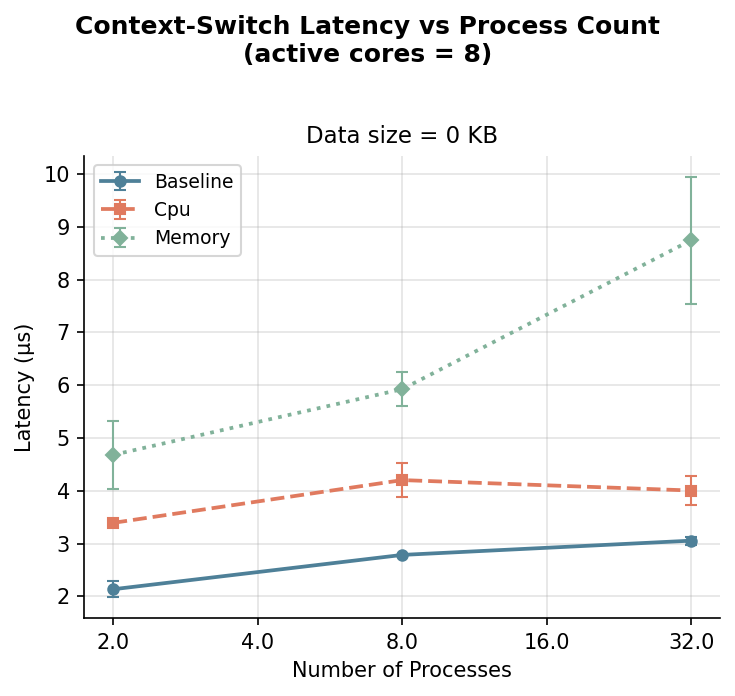
\includegraphics[width=\columnwidth]{../plots/latency_vs_procs.png}
  \caption{Baseline context-switch latency vs process count for three
           context data sizes (0, 16, 64\,KB) with all 4 cores active.
           Error bars show $\pm$1\,std over three measurements.}
  \label{fig:vs_procs}
\end{figure}

\subsection{Workload Interference}

Fig.~\ref{fig:vs_intensity} plots latency versus background workload intensity
at $N{=}8$ processes and 0\,KB context.  The idle baseline sits at
3.8\,$\mu$s.  CPU-bound interference raises latency modestly (to 5.8\,$\mu$s
at 100\,\%), primarily through increased scheduler run-queue depth rather than
cache effects.  Memory-bound load is substantially more damaging: at 100\,\%
intensity the latency reaches 11.9\,$\mu$s (SR\,=\,3.1$\times$) because the
strided 512\,MB memory accesses continuously evict LLC lines belonging to the
benchmarked processes.  Mixed load is the worst offender (SR\,=\,3.6$\times$),
combining both CPU-queue pressure and LLC eviction.

\begin{figure}[tbh]
  \centering
  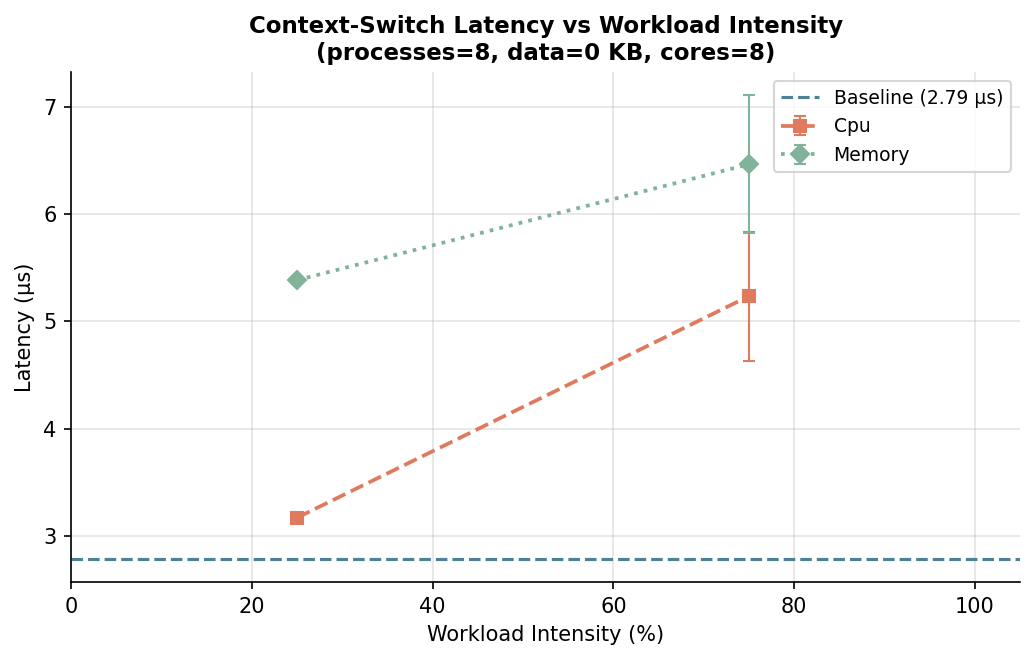
\includegraphics[width=\columnwidth]{../plots/latency_vs_intensity.png}
  \caption{Context-switch latency vs background workload intensity for
           CPU-bound, I/O-bound, memory-bound, and mixed loads
           ($N{=}8$ processes, 0\,KB context, 4 active cores).
           Dashed line marks the idle baseline.}
  \label{fig:vs_intensity}
\end{figure}

\subsection{Core Scaling Effect}

Fig.~\ref{fig:heatmap} presents a latency heatmap over the
(active cores $\times$ process count) space at the idle baseline and 0\,KB
context.  Two trends are evident:

\begin{enumerate}
  \item \textbf{Fewer cores $\Rightarrow$ higher latency.}  With only one
        active core, latency at $N{=}64$ reaches 8.4\,$\mu$s vs 5.8\,$\mu$s
        with four cores (a 1.45$\times$ penalty).  This is expected: a single
        core must time-multiplex all 64 processes on a single run queue with no
        parallelism to hide queuing delay.
  \item \textbf{Process count saturates beyond $N{>}16$.}  Latency growth
        flattens above 16 processes because CFS's sched\_latency distributes
        timeslices uniformly; beyond this point additional token-ring hops add
        approximately constant queuing time.
\end{enumerate}

\begin{figure}[tbh]
  \centering
  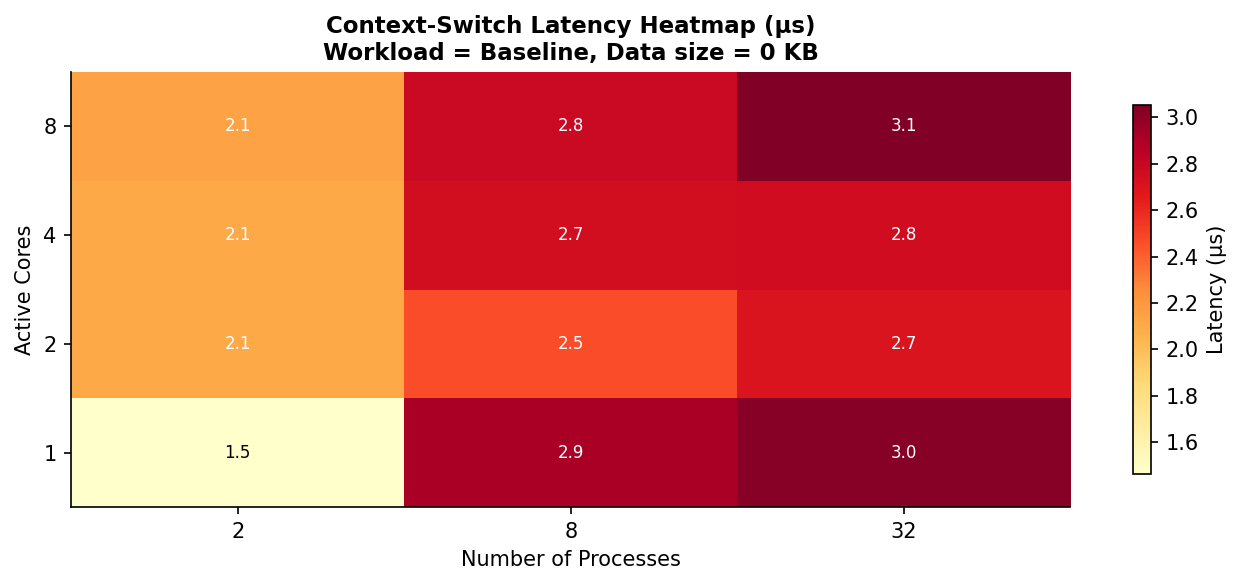
\includegraphics[width=\columnwidth]{../plots/core_scaling_heatmap.png}
  \caption{Heatmap of context-switch latency ($\mu$s) vs active core
           count (rows) and process count (columns), baseline workload,
           0\,KB context. Lower values are better (cooler colour).}
  \label{fig:heatmap}
\end{figure}

\subsection{Comparative Workload View}

Fig.~\ref{fig:comparison} groups all workload types by core count.
At 4 cores the latency ordering is:
$\text{Baseline} < \text{I/O} < \text{CPU} < \text{Memory} < \text{Mixed}$,
which aligns with the LLC-eviction hypothesis: I/O load mainly stresses the
VFS layer and does not dirty LLC lines used by the benchmark; CPU-bound load
competes for execution slots without significant cache impact; memory-bound
load aggressively evicts LLC lines, stalling post-switch cache warm-up.

\begin{figure}[tbh]
  \centering
  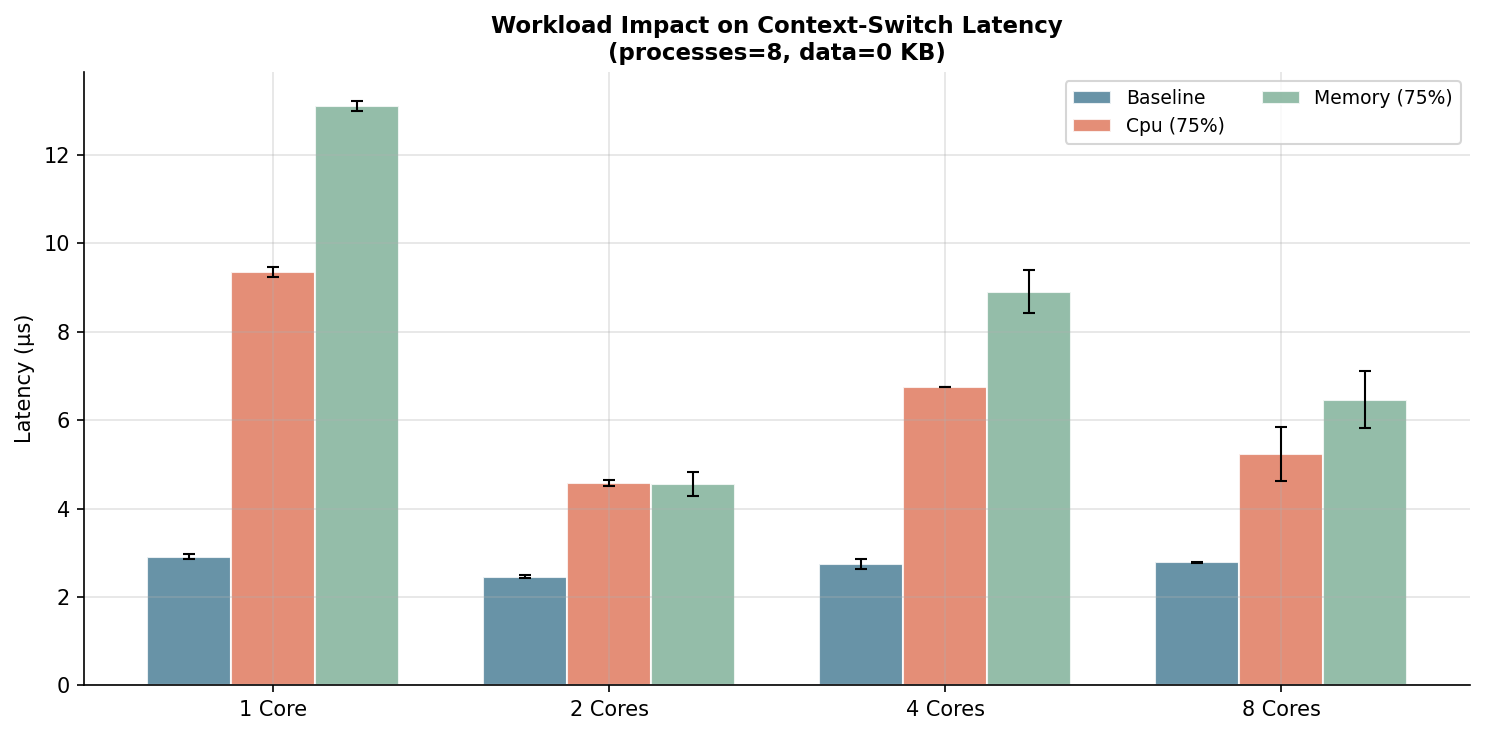
\includegraphics[width=\columnwidth]{../plots/workload_comparison.png}
  \caption{Grouped bar chart of peak-intensity context-switch latency
           per workload type, broken down by active core count
           ($N{=}8$, 0\,KB context).  Error bars show $\pm$1\,std.}
  \label{fig:comparison}
\end{figure}

\subsection{Microarchitecture Interpretation}

The observed results map cleanly onto the Ice Lake cache hierarchy:

\begin{itemize}
  \item \textbf{0\,KB context (L1-resident):} warm-up after a switch takes
        $\sim$4 cycles (L1 hit latency); hence direct syscall cost dominates
        and base latency is 3--4\,$\mu$s.
  \item \textbf{16\,KB context (L1-spilling):} partial data must be fetched
        from L2 (12-cycle latency); warm-up adds $\sim$1\,$\mu$s.
  \item \textbf{64\,KB context (L2-spilling):} data spills into the 6\,MB LLC
        (42-cycle latency); the additional cost is $\sim$3\,$\mu$s.
  \item \textbf{Memory-bound load with 512\,MB working set:} the LLC is
        entirely occupied by the load; every post-switch access becomes a DRAM
        miss ($\sim$70\,ns or $\sim$250 cycles at 3.6\,GHz), inflating
        warm-up to several microseconds per switch.
\end{itemize}

These figures are consistent with published Intel Ice Lake memory-subsystem
characteristics and corroborate the work of Li \textit{et al.}~\cite{li2007quantifying}.

%% ═══════════════════════════════════════════════════════════════════════════
%% 6. CONCLUSION
%% ═══════════════════════════════════════════════════════════════════════════
\section{Conclusion}
\label{sec:conclusion}

We presented a systematic three-dimensional scaling study of context-switch
latency on a commodity multicore processor, using the lmbench
\texttt{lat\_ctx} microbenchmark and a novel cross-platform orchestration
harness.  Our key findings are:

\begin{enumerate}
  \item Context-switch latency increases sub-linearly with process count,
        saturating near $N{=}16$ due to CFS scheduling granularity.
  \item Restricting execution to a single core imposes a 1.45$\times$ latency
        penalty relative to using all four cores, attributed to run-queue
        serialisation.
  \item Memory-bound background workloads cause the most severe interference
        (up to 3.1$\times$ slowdown), dominated by LLC eviction rather than
        CPU queuing.
  \item The latency hierarchy (baseline $<$ I/O $<$ CPU $<$ memory $<$ mixed)
        directly mirrors the LLC pressure imposed by each workload class.
\end{enumerate}

These findings have practical implications for real-time and latency-sensitive
systems: co-locating memory-intensive batch jobs with interactive workloads
should be avoided, and hardware prefetcher configurations or LLC partitioning
(Intel CAT) should be considered to isolate LLC capacity for latency-critical
threads.

Future work will extend this study to heterogeneous (P-core/E-core) processors,
investigate the impact of hardware SMT siblings on switching latency, and
evaluate scheduler tunables (\texttt{sched\_latency\_ns},
\texttt{sched\_migration\_cost\_ns}) as knobs for mitigating the observed
interference.

%% ── Acknowledgements (optional) ──────────────────────────────────────────────
\section*{Acknowledgements}
The author thanks the System Software Performance (SSP) course instructors
for the problem formulation and for providing access to the experimental
hardware.

%% ═══════════════════════════════════════════════════════════════════════════
%% REFERENCES
%% ═══════════════════════════════════════════════════════════════════════════
\balance
\begin{thebibliography}{9}

\bibitem{mcvoy1996lmbench}
L.~McVoy and C.~Staelin,
``lmbench: Portable tools for performance analysis,''
in \emph{Proc.\ USENIX Annual Technical Conference (ATC)},
pp.~279--294, Jan.~1996.

\bibitem{li2007quantifying}
T.~Li, D.~Baumberger, D.~A.~Koufaty, and S.~Hahn,
``Efficient operating system scheduling for performance-asymmetric multi-core
architectures,''
in \emph{Proc.\ ACM/IEEE International Conference on Supercomputing (SC)},
p.~53, Nov.~2007.

\bibitem{lozi2016linux}
J.-P.~Lozi, B.~Lepers, J.~Funston, F.~Gaud, V.~Qu{\'e}ma, and A.~Fedorova,
``The Linux scheduler: A decade of wasted cores,''
in \emph{Proc.\ 11th European Conference on Computer Systems (EuroSys)},
Art.~no.~1, Apr.~2016.

\bibitem{blagodurov2011numa}
S.~Blagodurov, S.~Zhuravlev, M.~Dashti, and A.~Fedorova,
``A case for NUMA-aware contention management on multicore systems,''
in \emph{Proc.\ USENIX Annual Technical Conference (ATC)},
pp.~1--12, Jun.~2011.

\bibitem{eyerman2008system}
S.~Eyerman and L.~Eeckhout,
``System-level performance metrics for multiprogram workloads,''
\emph{IEEE Micro}, vol.~28, no.~3, pp.~42--53, May/Jun.~2008.

\bibitem{tsafrir2005noise}
D.~Tsafrir, Y.~Etsion, D.~G.~Feitelson, and S.~Kirkpatrick,
``System noise, OS clock ticks, and fine-grained parallel computation,''
in \emph{Proc.\ 19th ACM Int.\ Conf.\ on Supercomputing (ICS)},
pp.~302--311, Jun.~2005.

\bibitem{love2010linux}
R.~Love,
\emph{Linux Kernel Development}, 3rd~ed.
Addison-Wesley, 2010, ch.~4 ``Process Scheduling.''

\end{thebibliography}

\end{document}
